\documentclass{article}
\usepackage[utf8]{inputenc}
\usepackage{amsmath}
\usepackage{amssymb}
\usepackage{amsthm}
\usepackage{cancel}
\usepackage[shortlabels]{enumitem}
\usepackage{caption}
\usepackage{graphicx}
\usepackage[top=0.5in, bottom=0.5in, left=1in, right=1in]{geometry}
\usepackage{float}

% \usepackage{titlesec}
%     \titlespacing{\subsection}{\parindent}{15pt}{12pt}

\title{\textbf{\underline{CSCI3070U: Analysis \& Design of Algorithms}\\Greedy Algorithms}}
\author{Syed Naqvi\\100590852}
\date{\today}

\begin{document}

    \maketitle
    
    \subsection*{A)}

    \begin{center}
        \begin{minipage}[t]{0.9\textwidth}
            Fractional solution for knapsack with maximum weight 25 and provided items:
            \begin{figure}[H]
                \centering
                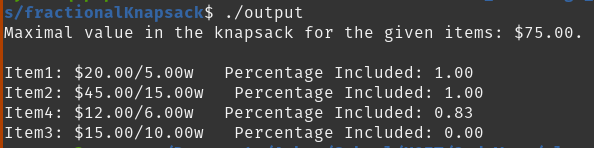
\includegraphics[width=0.7\textwidth, height=0.1\textheight]{./parta.png}
            \end{figure}
        \end{minipage}
    \end{center}

    \subsection*{B)}

    \begin{center}
        \begin{minipage}[t]{0.9\textwidth}
            Using Huffman's algorithm to find the encodings for the provided characters and frequencies.
            Determining the file length for for Huffman codes and fixed codes. 
            \begin{figure}[H]
                \centering
                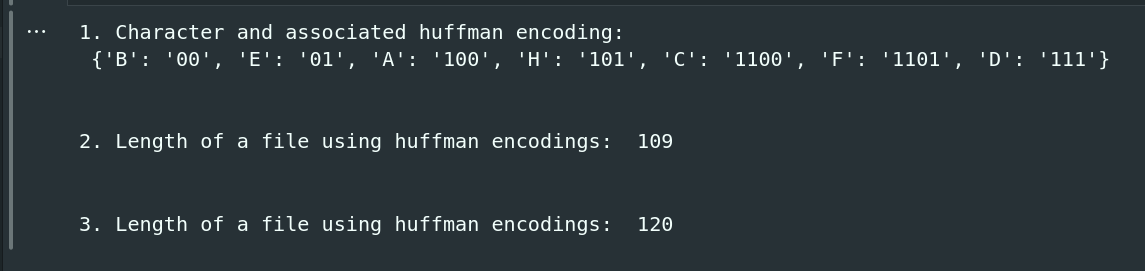
\includegraphics[width=0.7\textwidth, height=0.1\textheight]{./partb.png}
            \end{figure}
        \end{minipage}
    \end{center}

    \subsection*{C)}

    \begin{center}
        \begin{minipage}[t]{0.9\textwidth}
            See full implementation using C++:
            \begin{figure}[H]
                \centering
                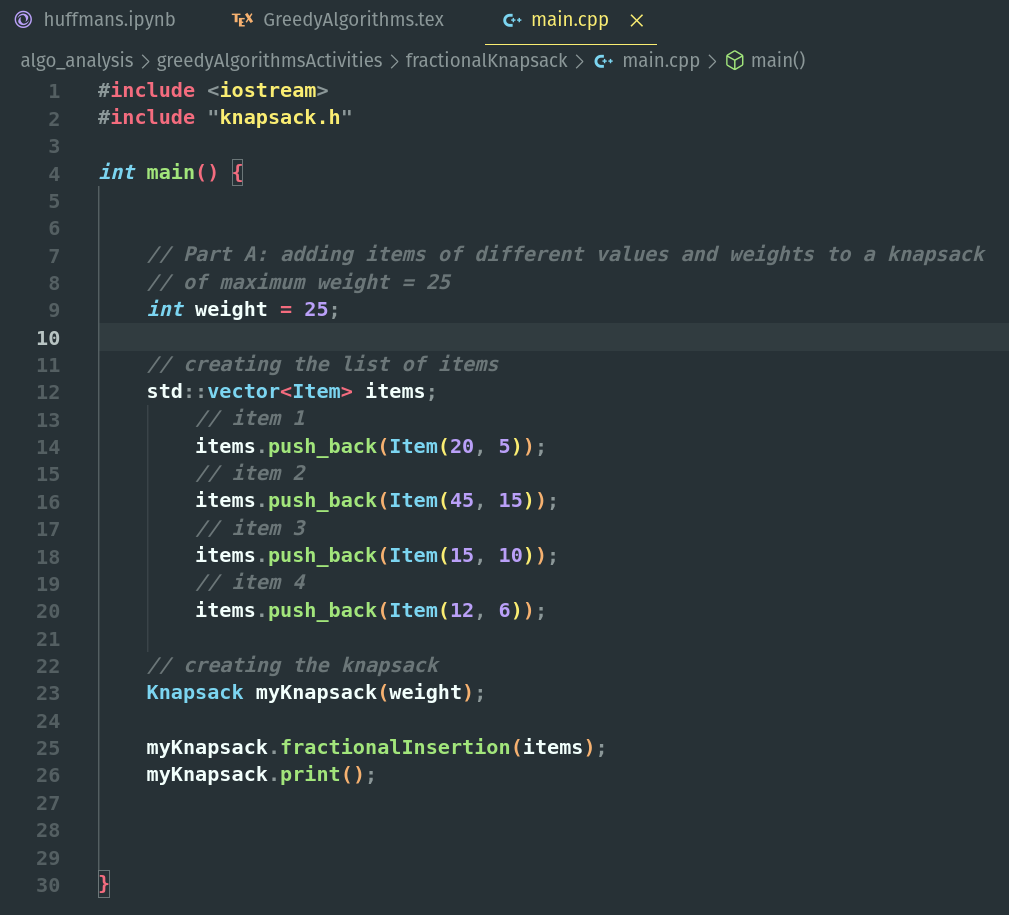
\includegraphics[width=0.9\textwidth, height=0.5\textheight]{./partc.png}
            \end{figure}
        \end{minipage}
    \end{center}

\end{document}